% ── SLIDE 3: CBS Block ──────────────────────────────────────────────
\begin{frame}{YOLOv11: Conv + BatchNorm + SiLU Block}
  \centering
  \begin{columns}[c]
    \begin{column}{0.39\textwidth}
      \centering
      \begin{tikzpicture}[
          cbsbox/.style={
              draw=utecblue!85,
              fill=utecblue!5,
              rounded corners=15pt,
              line width=1.2pt,
              minimum width=3.25cm,
              minimum height=5.25cm
            },
          layer/.style={
              draw=utecblue!85,
              fill=white,
              rounded corners=7pt,
              line width=1.0pt,
              minimum width=2.45cm,
              minimum height=0.66cm,
              font=\small\bfseries,
              align=center
            },
          arr/.style={-{Stealth[length=5pt]}, utecblue!80, line width=1.0pt}
        ]
        \node[cbsbox] (outer) at (0,0) {};
        \node[font=\Large\bfseries, text=utecblue!90] at (0,2.12) {CBS};
        \node[layer] (conv) at (0,1.15) {Conv2d};
        \node[layer] (bn) at (0,0.0) {BatchNorm2d};
        \node[layer] (silu) at (0,-1.15) {SiLU};
        \draw[arr] (conv) -- (bn);
        \draw[arr] (bn) -- (silu);
      \end{tikzpicture}
    \end{column}
    \begin{column}{0.57\textwidth}
      \centering
      \[
        \mathrm{SiLU}(x)=x\cdot\frac{1}{1+e^{-x}}
      \]
      \vspace{0.2cm}
      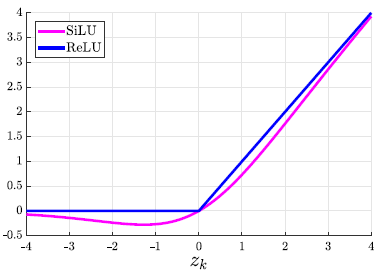
\includegraphics[width=0.9\linewidth]{figures/silu.png}
    \end{column}
  \end{columns}
\end{frame}

